 \documentclass{beamer}

\usetheme{MagdeburgFIN}
\usefonttheme{structurebold}
\usepackage{graphicx}
\usepackage{float}
\usepackage{url}
\usepackage{pdfpages}


\title{SIMD Acceleration for Index Structures}
\author{Marten Wallewein-Eising}
\date{\today}
\institute{Otto von Guericke Univerity, Magdeburg}

\begin{document}

\begin{frame}[plain]
 \titlepage
\end{frame}



\section[Agenda]{}
\begin{frame}
\frametitle{Agenda}
\tableofcontents
\end{frame}

\section{Motivation}
\begin{frame}
\frametitle{Motivation}
TODO: Insert Big Picture here...
\end{frame}

\section{Short information about B$^{+}$- and Radix-Trees}
\begin{frame}
\frametitle{B$^{+}$-Tree}
	\begin{center}
		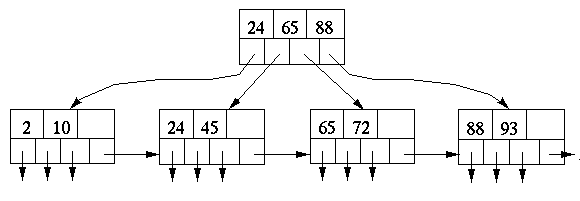
\includegraphics[width=0.8\textwidth]{img/b_tree.png}
	\end{center}
	\begin{itemize}
		\item N-ary tree with large number of children per node
		\item Only leaf nodes contain values, inner nodes only children
		\item Leaf nodes often linked for range based scans
	\end{itemize}
\end{frame}
\begin{frame}
\frametitle{Radix-Tree}
	\begin{center}
	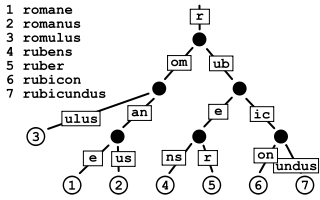
\includegraphics[width=0.6\textwidth]{img/radix_tree.png}
	\end{center}
	\begin{itemize}
		\item Space optimized prefix tree
		\item Number of children of every inner node is at least the radix $r$
		\item Each node that is the only child is merged with its parent
	\end{itemize}

\end{frame}
\section{SIMD Style Processing}
\begin{frame}
\frametitle{Single Instruction Multiple Data}
\begin{center}
	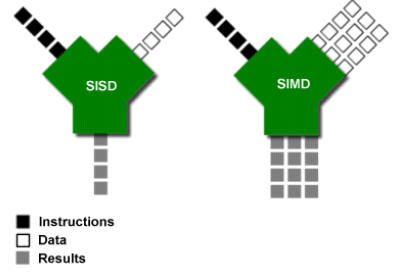
\includegraphics[width=0.6\textwidth]{img/simd.png}
\end{center}
\begin{itemize}
	\item \textbf{\_\_m128i \_mm\_cmpgt\_epi32 (\_\_m128i a, \_\_m128i b)} Compares 4 signed 32-bit integers in a and 4 signed 32-bit integers
	in b for greater-than.
\end{itemize}
\end{frame}
\begin{frame}
\frametitle{Horizontal Vectorization}
\begin{center}
	TODO: Insert Graphic here
\end{center}
\end{frame}
\section{Adapted Tree structures}

\subsection{Seg-Tree/Trie}

\subsection{FAST}

\subsection{VAST}

\subsection{ART}

\section{Evaluation}

\begin{frame}
\frametitle{Evaluation}
Implementation of the considered performance criteria and their impact:
\begin{figure}
	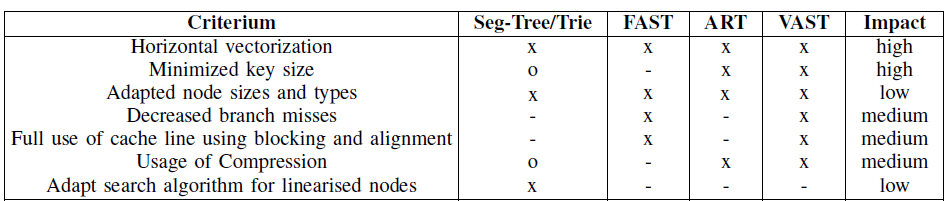
\includegraphics[width=1.05\textwidth]{img/table_eval.png}
\end{figure}
Legend: x: implements the issue, o: partially implements the issue, -: not implements the issue
\end{frame}

\begin{frame}
\frametitle{Sources}
\begin{itemize}
	\item http://infolab.stanford.edu/~nsample/cs245/handouts/hw2sol/sol2.html
	\item https://en.wikipedia.org/wiki/Radix\_tree
\end{itemize}
\end{frame}

\begin{frame}
 \frametitle{Thank you for your attention!}
\end{frame}
\end{document}
